         \chapter{Transversale golwe}\fancyfoot[LO,RE]{Fisika: Golwe, Klank en Lig}
    \setcounter{figure}{1}
    \setcounter{subfigure}{1}
    \label{m38806}
    \section{Inleiding}
            \nopagebreak
      \label{m38806*id317331}Golwe kom dikwels voor in die natuur. Die mees voor die hand liggende voorbeelde is golwe in die water; op 'n dam, in die see of in 'n emmer. Ons is geïnteresseerd in die eienskappe van golwe. Alle golwe het dieselfde eienskappe.
Golwe kom nie net in water voor nie, maar hulle kom ook in ander mediums voor. Aardbewings laat genoeg energie vry om golwe te inisieer wat sterk genoeg is om deur rotse in die aardkors te beweeg. Wanneer jou vriende met jou praat, word klankgolwe geproduseer wat deur die lug beweeg tot by jou ore. 'n Golf is, kortliks saamgevat, die versteuring van  'n medium deur die beweging van energie, maar hoe verskil dit van  'n puls?
\chapterstartvideo{VPgio}
    \section{Wat is 'n transversale golf?}

            \nopagebreak
\begin{minipage}{.5\textwidth}
\textbf{Golwe in 'n swembad}\par
 \includegraphics[width=.8\textwidth]{photos/kreepykrawly.jpg}
\end{minipage}
\begin{minipage}{.5\textwidth}  
Ons het pulse bestudeer in die gedeelte oor \textit{Transversale pulse} en weet dat  'n puls  'n enkele versteuring is wat deur  'n medium beweeg. 'n \textsl{Golf} is 'n periodieke volgehoue versteuring wat bestaan uit  'n reeks opeenvolgende pulse. 'n Vergrote weergawe van  'n golftenk kan word  gesien word in die alledaagse voorbeeld van 'n Kreepy Krauly\textregistered\ wat golwe veroorsaak in  'n swembad as gevolg van sy reelmatige vibrasies. Die Kreepy Krauly\textregistered\ is ontwikkel in Suid-Afrika deur Ferdinand Chauvier en sy seun Daniel.\\
\end{minipage}
% \label{m38806*fhsst!!!underscore!!!id83}\begin{definition}
	  \Definition{Golf} {n Golf is 'n periodieke volgehoue versteuring wat bestaan ​​uit opeenvolgende pulse.} 
\Definition{ Transversale golf} { 'n Transversale golf is 'n golf waar die beweging van die deeltjies van die medium loodreg (reghoekig) is op die voortplantingsrigting van die golf.} 

\label{m38806*secfhsst!!!underscore!!!id89}
            \begin{activity}{Transversale golwe}
            \nopagebreak
      \label{m38806*id317764}
Gebruik  'n tou of  'n opgerolde veer ( 'n “slinky”). Strek die tou of veer horisontaal uit en laat twee persone aan elke kant vashou. Beweeg die een kant van die tou vinnig op en af om  'n reeks pulse te veroorsaak en hou vir  'n ruk aan met die beweging.\\
      \label{m38806*id317781}
    \setcounter{subfigure}{0}
	\begin{figure}[H] % horizontal\label{m38806*id317784}
    \begin{center}
\begin{pspicture}(0,-1.2546875)(7.62,1.2346874)
\psline[linewidth=0.04cm](1.6,0.5146875)(7.6,0.5146875)
\psline[linewidth=0.04cm](1.6,0.2146875)(7.6,0.2146875)
\psline[linewidth=0.02cm](1.64,0.5146875)(1.94,0.2146875)
\psline[linewidth=0.02cm](2.24,0.5146875)(2.54,0.2146875)
\psline[linewidth=0.02cm](2.84,0.5146875)(3.14,0.2146875)
\psline[linewidth=0.02cm](4.04,0.5146875)(4.34,0.2146875)
\psline[linewidth=0.02cm](3.44,0.5146875)(3.74,0.2146875)
\psline[linewidth=0.02cm](4.64,0.5146875)(4.94,0.2146875)
\psline[linewidth=0.02cm](5.24,0.5146875)(5.54,0.2146875)
\psline[linewidth=0.02cm](5.84,0.5146875)(6.14,0.2146875)
\psline[linewidth=0.02cm](6.44,0.5146875)(6.74,0.2146875)
\psline[linewidth=0.02cm](7.04,0.5146875)(7.34,0.2146875)
\psline[linewidth=0.04cm,arrowsize=0.1029cm 3.0,arrowlength=1.6,arrowinset=0.4]{<-}(1.2,-0.4853125)(1.2,1.2146875)
\psline[linewidth=0.04cm,arrowsize=0.1029cm 3.0,arrowlength=1.6,arrowinset=0.4]{->}(0.8,-0.4853125)(0.8,1.2146875)
\psline[linewidth=0.04cm,arrowsize=0.1029cm 3.0,arrowlength=1.6,arrowinset=0.4]{<-}(0.4,-0.4853125)(0.4,1.2146875)
\psline[linewidth=0.04cm,arrowsize=0.1029cm 3.0,arrowlength=1.6,arrowinset=0.4]{->}(0.0,-0.4853125)(0.0,1.2146875)
%\usefont{T1}{ptm}{m}{n}
\rput(2.1485937,-1.0353125){Beweeg tou op en af}
\end{pspicture}
\end{center}
 \end{figure}       
      \par 
      \label{m38806*id317791}\begin{enumerate}[noitemsep, label=\textbf{\arabic*}. ] 
            \label{m38806*uid1}\item Beskryf wat gebeur met die tou.
\label{m38806*uid2}\item Maak  'n skets om aan te toon hoe die tou lyk terwyl die pulse daardeur beweeg.
\label{m38806*uid3}\item In watter rigting beweeg die pulse?
\label{m38806*uid4}\item Bind 'n lint in die middel van die tou. Dit dui 'n deeltjie in die tou aan.
    \setcounter{subfigure}{0}
	\begin{figure}[H] % horizontal\label{m38806*id317844}
   \begin{center}
\begin{pspicture}(0,-1.2446876)(7.64,1.2446876)
\psline[linewidth=0.04cm](1.62,0.5246875)(7.62,0.5246875)
\psline[linewidth=0.04cm](1.62,0.2246875)(7.62,0.2246875)
\psline[linewidth=0.02cm](1.66,0.5246875)(1.96,0.2246875)
\psline[linewidth=0.02cm](2.26,0.5246875)(2.56,0.2246875)
\psline[linewidth=0.02cm](2.86,0.5246875)(3.16,0.2246875)
\psline[linewidth=0.02cm](4.06,0.5246875)(4.36,0.2246875)
\psline[linewidth=0.02cm](3.46,0.5246875)(3.76,0.2246875)
\psline[linewidth=0.02cm](4.66,0.5246875)(4.96,0.2246875)
\psline[linewidth=0.02cm](5.26,0.5246875)(5.56,0.2246875)
\psline[linewidth=0.02cm](5.86,0.5246875)(6.16,0.2246875)
\psline[linewidth=0.02cm](6.46,0.5246875)(6.76,0.2246875)
\psline[linewidth=0.02cm](7.06,0.5246875)(7.36,0.2246875)
\psline[linewidth=0.04cm,arrowsize=0.1029cm 3.0,arrowlength=1.6,arrowinset=0.4]{<-}(1.22,-0.4753125)(1.22,1.2246875)
\psline[linewidth=0.04cm,arrowsize=0.1029cm 3.0,arrowlength=1.6,arrowinset=0.4]{->}(0.82,-0.4753125)(0.82,1.2246875)
\psline[linewidth=0.04cm,arrowsize=0.1029cm 3.0,arrowlength=1.6,arrowinset=0.4]{<-}(0.42,-0.4753125)(0.42,1.2246875)
\psline[linewidth=0.04cm,arrowsize=0.1029cm 3.0,arrowlength=1.6,arrowinset=0.4]{->}(0.02,-0.4753125)(0.02,1.2246875)
%\usefont{T1}{ptm}{m}{n}
\rput(2.1685936,-1.0253125){Beweeg tou op en af}
\psline[linewidth=0.08cm](4.52,0.5246875)(4.52,0.2246875)
\psbezier[linewidth=0.06](4.624195,0.5223207)(4.5021477,0.5799539)(4.558249,0.5731951)(4.604037,0.69499725)(4.649824,0.81679934)(4.7504873,0.9280784)(4.8152437,0.84101325)(4.88,0.75394803)(4.7462425,0.4646875)(4.624195,0.5223207)
\psline[linewidth=0.06cm](4.52,0.5446875)(4.84,0.1046875)
\psline[linewidth=0.06cm](4.5,0.4646875)(4.3,0.1246875)
\psbezier[linewidth=0.06](4.4578786,0.45692405)(4.6,0.50916064)(4.534671,0.5030347)(4.481353,0.6134316)(4.4280343,0.7238284)(4.3108144,0.8246875)(4.2354074,0.7457749)(4.16,0.6668623)(4.3157578,0.4046875)(4.4578786,0.45692405)
\end{pspicture}
\end{center}

 \end{figure}       \label{m38806*uid5}\item Beweeg die tou vir  'n volgehoue tyd. Hou die lint fyn dop terwyl die pulse deur die tou beweeg. Beskryf wat gebeur met die lint.
\label{m38806*uid6}\item Maak  'n skets om die beweging van die lint aan te toon. Dui die lint aan met  'n kolletjie en gebruik pyltjies om die beweging aan te dui. 
\end{enumerate}

\end{activity}

 In hierdie aktiwiteit het jy golwe veroorsaak. Die medium waardeur hierdie golwe voortgeplant is, was die tou, wat natuurlik bestaan ​​uit 'n baie groot aantal deeltjies (atome). Vanuit die aktiwiteit kan jy aflei dat die golf beweeg het van die een kant na die ander kant van die tou, maar dat die deeltjies (die lint) slegs op en af beweeg het. \\
    \setcounter{subfigure}{0}
	\begin{figure}[H] % horizontal\label{m38806*uid7}
%    \begin{center}
%    \rule[.1in]{\figurerulewidth}{.005in} \\
%        \label{m38806*uid7!!!underscore!!!media}\label{m38806*uid7!!!underscore!!!printimage}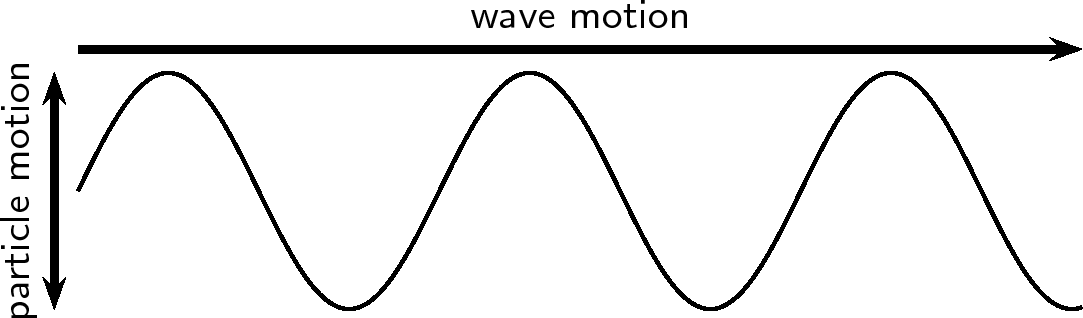
\includegraphics[width=300px]{col11305.imgs/m38806_PG10C5_003.png} % m38806;PG10C5\_003.png;;;6.0;8.5;
%      \vspace{2pt}
%    \vspace{\rubberspace}\par \begin{cnxcaption}
%	  \small \textbf{Figure 7.3: }A transverse wave, showing the direction of motion of the wave perpendicular to the direction in which the particles move.
%	\end{cnxcaption}
%    \vspace{.1in}
%    \rule[.1in]{\figurerulewidth}{.005in} \\
%    \end{center}
\begin{center}
\begin{pspicture}(-0.6,-1.6)(9,1.6)
%\psgrid
\psplot[xunit=0.017,plotpoints=300]{0}{500}{x 2 mul sin}
\psline[linewidth=2pt]{<->}(-0.2,-1)(-0.2,1)
\rput{90}(-0.5,0){deeltjiebeweging}
\psline[linewidth=2pt]{->}(0,1.2)(8.5,1.2)
\uput[u](4.25,1.2){golfbeweging}
\end{pspicture}
\caption{ 'n Transversale golf, waar aangedui word dat die rigting van die golfbeweging loodreg is op die rigting waarin die deeltjies beweeg.}
\label{m38806*uid7!!!underscore!!!media}
\end{center} 


\end{figure}       
Wanneer die deeltjies van die medium loodreg beweeg op die voortplantingsrigting van die golf, is dit  'n transversale golf. By golwe is daar geen netto verplasing van die deeltjies van die medium nie (hulle keer terug na hulle na hulle ewewigsposisie), maar daar is 'n netto verplasing van die golf. Daar is dus twee verskillende bewegings: die beweging van die deeltjies van die medium en die beweging van die golf.\\
Die volgende simulasie sal jou help om meer te verstaan oor golwe. Kies die ossileer-opsie
    en neem waar wat gebeur.

\simulation{Transversale golwe}{P10042}

\par \label{m38806*uid8}
            \section{Kruine en buike}
            \nopagebreak
        \label{m38806*id317923}Golwe het bewegende kruine en buike. 'n Kruin is die hoogste punt wat die medium bereik as die golf deurbeweeg en die buik is die laagste punt tot waar die medium daal.\\
       Kruine en buike word aangetoon op 'n transversale golf in Figuur~\ref{fig:p:wsl:tw10:transverse:peaktrough}.

\begin{figure}[htbp]
\begin{center}
\begin{pspicture}(-4,-1.1)(6,1.1)
%\psgrid
\psplot[xunit=0.0055,yunit=0.5,plotpoints=300]{-720}{720}{x sin }
\psline[linestyle=dashed](-4,0)(4,0)
\psline{<-}(4.1,0)(4.7,0)
\rput[l](4.8,0){ewewigsposisie}
\rput[l](4.3,1){Kruine}
\psline{<-}(-1.483,0.55)(-1.483,1)(3.5,1)
\psline{<-}(.497,0.55)(.497,1)(3.5,1)
\psline{<-}(2.477,0.55)(2.477,1)(3.5,1) \rput[l](4.3,-1){Buike}
\psline{<-}(1.487,-0.55)(1.487,-1)(3.3,-1)
\psline{<-}(-.493,-0.55)(-.493,-1)(3.3,-1)
\psline{<-}(-2.473,-0.55)(-2.473,-1)(3.3,-1)
\end{pspicture}
\caption{Kruine en buike in 'n transversale golf.}
\label{fig:p:wsl:tw10:transverse:peaktrough}
\end{center}
\end{figure}
      
\par
\Definition{Kruine en buike} {  'n Kruin is 'n punt op  'n golf waar die verplasing van die medium by 'n  maksimum is.
       'n Buik is  'n punt op  'n  golf waar die verplasing van die medium by  'n minimum is. } 
      \label{m38806*uid10}
\section{Amplitude}
\begin{activity}{Amplitude}
\begin{center}
\begin{pspicture}(-2,-1.4)(6,1.4)
%\psgrid
\def\halfwave{\psplot[xunit=0.0055,plotpoints=1200]{0}{1080}{x sin 1.4 mul}}
\rput(0,0){\halfwave\psline{<->}(0.5,0)(0.5,1.4)}
%\rput(0.7,0.875){a}
\psline[linestyle=dashed](0,0)(6,0)\uput[l](0,0){ewewigsposisie}

\rput(0,0){\halfwave\psline{<->}(0.5,0)(0.5,1.4)\uput[r](0.4,0.6){a}}
\rput(2,0){%\rput[l]{180}{\halfwave}
\psline{<->}(-0.515,0)(-0.515,-1.4)\uput[r](-0.6,-0.6){b}}
\rput(2,0){%\halfwave
\psline{<->}(0.48,0)(0.48,1.4)\uput[r](0.4,0.6){c}}
\rput(4,0){%\rput[l]{180}{\halfwave}
\psline{<->}(-0.535,0)(-0.535,-1.4)\uput[r](-0.6,-0.6){d}}
\rput(4,0){%\halfwave
\psline{<->}(0.455,0)(0.455,1.4)\uput[r](0.4,0.6){e}}
\rput(6,0){%\rput[l]{180}{\halfwave}
\psline{<->}(-0.565,0)(-0.565,-1.4)\uput[r](-0.6,-0.6){f}}
\psline[linestyle=dashed](0,0)(6,0)\uput[l](0,0){ewewigsposisie}
\end{pspicture}
\end{center}

Voltooi die onderstaande tabel deur die meting van die afstand tussen die ewewigsposisie en elke kruin en die buik in die golf hierbo. Gebruik jou liniaal om die afstande te meet.

\begin{center}
\begin{tabular}{|c|c|}\hline
Kruin/Trog&Meting (cm)\\\hline
a&\\\hline
b&\\\hline
c&\\\hline
d&\\\hline
e&\\\hline
f&\\\hline
\end{tabular}
\end{center}

\begin{enumerate}[noitemsep, label=\textbf{\arabic*}. ]
\item Wat kan jy s\^{e} oor jou resultate?
\item Is die afstande tussen die ewewigsposisie en elke kruin dieselfde?
\item Is die afstande tussen die ewewigsposisie en elke buik dieselfde?
\item Is die afstand tussen die ewewigsposisie en die kruin gelyk aan die afstand tussen die ewewigsposisie en die trog?
\end{enumerate}
\end{activity}

\IFact{'n Tsoenamie is 'n reeks van die seegolwe wat veroorsaak word deur 'n onderwater aardbewing,   grondverskuiwing of vulkaniese uitbarsting. Wanneer die see diep is, kan tsoenamies minder as 30 cm
    hoog op die oppervlak van die oseaan beweeg teen 'n spoed van tot $700 \text{ km} \cdot \text{ h}^{-1}$. In vlak
    water naby die kus beweeg dit stadiger. Die bopunt van die golf beweeg vinniger as die onderkant en dit 
    veroorsaak dat die see dramaties styg, tot soveel as 30 m. Die golflengte kan so lank
    as 100 km wees en die periode kan tot so lank as 'n uur wees.}
Soos ons gesien het in die aktiwiteit oor amplitude, is die afstand tussen die kruin en die ewewigsposisie gelyk aan die afstand tussen die buik en die ewewigsposisie. Hierdie afstand staan ​​bekend as die amplitude van die golf en is die kenmerkende hoogte van die golf, bo- of onderkant die ewewigsposisie. Normaalweg word die simbool A gebruik om die \textsl{amplitude} van 'n golf te verteenwoordig. Die SI-eenheid van amplitude is die meter (m).
\Definition{ Amplitude } {Die amplitude van 'n golf is 'n aanduiding van die afstand wat die medium verplaas word vanaf die ewewigsposisie (rusposisie). \\ 
Hoeveelheid: Amplitude (A) \hspace{.5cm} Eenheid naam: meter \hspace{.5cm} Eenheid simbool: $m$}
        \label{m38806*id318448}
    \setcounter{subfigure}{0}
	\begin{figure}[H] % horizontal\label{m38806*id318451}
    \begin{center}
\begin{pspicture}(-5,-1)(5,1)%\psgrid
\psplot[xunit=0.0055,]{-360}{360}{x sin }
\psline[linestyle=dashed](-3,0)(3,0)
\rput(4,0.5){Amplitude}
\psline{<->}(3.,0)(3.,1)
\rput(4,-.5){Amplitude}
\psline{<->}(3.,0)(3.,-1)
\psline[linestyle=dashed](.495,1)(3,1)
\psline[linestyle=dashed](1.485,-1)(3,-1)
\psline{<->}(-3,-1)(-3,1)
\rput(-4.5,0){2 x Amplitude}
\end{pspicture}
\end{center}
 \end{figure}       
        \par 
\label{m38806*secfhsst!!!underscore!!!id212}\vspace{.5cm} 

 In 2004 is die Indiese Oseaan-tsoenamie veroorsaak deur 'n aardbewing wat dieselfde energie as sowat
    23 000 atoombomme gehad het. Binne enkele ure na die aardbewing het dodelike golwe, uitgestraal vanaf die aardbewing, die kuslyn van 11 lande getref en gelei tot die dood van ongeveer 150 000 mense. Die finale dodetal was 283 000.
\vspace{-1cm}
\begin{wex}
{%title
Amplitude van die seegolwe
}
{%question
As die kruin van 'n golf  $2~\text{m}$ bokant die stilwatermerk in  'n hawe gemeet kan word , wat
    die amplitude van die golf?
}
{%solution
\westep{Ontleed die inligting wat gegee is}{
Ons is vertel dat die hawe 'n stilwaterpunt het. Dit is 'n lyn wat aandui wat die watervlak is wanneer daar geen versteurings in die water is nie en wat dus die ewewigsposisie verteenwoordig.
}
\westep{Bepaal die amplitude}{  
 Die definisie van die amplitude is die maksimum hoogte van  'n kruin bokant die ewewigsposisie. Die stilwaterpunt is die hoogte van die water by die ewewigsposisie en die kruin is $2\phantom{\rule{2pt}{0ex}}\text{m}$ bokant hierdie
      posisie, dus is die amplitude $2\phantom{\rule{2pt}{0ex}}\text{m}$. 
}
}
\end{wex}
    

\noindent
\label{m38806*secfhsst!!!underscore!!!id221}
            \begin{activity}{Golflengte}
            \nopagebreak
        \label{m38806*id318517}
    \setcounter{subfigure}{0}
	\begin{figure}[H] % horizontal\label{m38806*id318520}
    \begin{center}
\scalebox{.8}{
\begin{pspicture}(-2,-2.6)(6,2.6)
%\psgrid%[gridcolor=lightgray]
\psplot[xunit=0.00555556,plotpoints=300]{0}{1080}{x sin 1.8 mul}
\pcline[offset=-8pt]{|-|}(1.5,-1.8)(3.5,-1.8)
\bput{:U}{a}
\pcline[offset=-8pt]{|-|}(3.5,-1.8)(5.5,-1.8)
\bput{:U}{b}
\pcline[offset=8pt]{|-|}(0.5,1.8)(2.5,1.8)
\aput{:U}{c}
\pcline[offset=8pt]{|-|}(2.5,1.8)(4.5,1.8)
\aput{:U}{d}
\psline[linestyle=dashed](0,0)(6,0)\uput[l](0,0){ewewigsposisie}
\end{pspicture}}
\end{center} \end{figure}       
        \par 
Voltooi die onderstaande tabel deur die meting van die afstand tussen die kruine en buike in die
       golf hierbo.
    % \textbf{m38806*id318530}\par
\begin{center}
\begin{tabular}{|c|c|}\hline
&Afstand(cm)\\\hline
a&\\\hline
b&\\\hline
c&\\\hline
d&\\\hline
\end{tabular}
\end{center}
    \par
        \label{m38806*id318631}\begin{enumerate}[noitemsep, label=\textbf{\arabic*}. ] 
            \label{m38806*uid15}\item Wat kan jy s\^{e} oor jou resultate?
\label{m38806*uid16}\item Is die afstande tussen kruine dieselfde?
\label{m38806*uid17}\item Is die afstande tussen buike dieselfde?
\label{m38806*uid18}\item Is die afstand tussen die kruine gelyk aan die afstand tussen die buike?
\end{enumerate}

\end{activity}

 Soos ons gesien het in die aktiwiteit oor golflengte, is die afstand tussen twee aangrensende
    kruine dieselfde ongeag watter twee aangrensende kruine jy kies om te meet. Die afstand tussen twee 
    opeenvolgende kruine is dus konstant. Net so sien ons dat die afstand tussen twee opeenvolgende buike
    dieselfde bly, ongeag watter twee buike jy kies om te meet.  'n Verdere belangrike afleiding om te maak, is dat
    die afstand tussen twee opeenvolgende kruine dieselfde is as die afstand tussen twee opeenvolgende buike.
    Hierdie  afstand staan ​​bekend as die golflengte van die golf.\\
        \label{m38806*id318708}Die simbool vir golflengte is $\lambda $ (die Griekse letter \textsl{lambda}) en golflengte word gemeet in meter ($\text{m}$).\par 
        \label{m38806*id318725}
    \setcounter{subfigure}{0}
	\begin{figure}[H] % horizontal\label{m38806*id318728}
   \begin{center}
\begin{pspicture}(-2,-1.1)(2,1.1)
%\psgrid
\psplot[xunit=0.0055,]{-360}{360}{x sin}
\psline[linestyle=dashed](-3,0)(3,0)
\rput(-.5,1.35){$\lambda$}
\psline{<->}(0.495,1.06)(-1.485,1.06)
\rput(0.5,-1.35){$\lambda$}
\psline{<->}(-0.495,-1.06)(1.485,-1.06)
\end{pspicture}
\end{center} \end{figure}       
        \par 


\begin{wex}{Golflengte}{ Die totale afstand tussen 4 opeenvolgende kruine van 'n transversale golf is 6 m. Wat is
    die golflengte van die golf?}{
\westep{Teken 'n rowwe skets om die situasie voor te stel}

\begin{center}
\begin{pspicture}(-2,-2)(8,2.6)
%\psgrid%[gridcolor=lightgray]
\psplot[xunit=0.00555556,plotpoints=300]{0}{1440}{x sin 1.8 mul}
\pcline[offset=16pt]{|-|}(0.5,1.8)(6.5,1.8)
\aput{:U}{6\,m}
\psline[linestyle=dashed](0,0)(8,0)\uput[l](0,0){ewewigsposisie}
\pcline[offset=8pt]{|-|}(0.5,1.8)(2.5,1.8)
\bput{:U}{$\lambda$}
\pcline[offset=8pt]{-|}(2.5,1.8)(4.5,1.8)
\bput{:U}{$\lambda$}
\pcline[offset=8pt]{-|}(4.5,1.8)(6.5,1.8)
\bput{:U}{$\lambda$}

\end{pspicture}
\end{center}

\westep{Bepaal hoe om die probleem te benader}
Vanuit die skets kan ons sien dat 4 opeenvolgende kruine gelykstaande is aan 3 golflengtes.

\westep{Los die probleem op}
Daarom is die golflengte van die golf gelyk aan:
\begin{eqnarray*}
3\lambda&=&6~\text{m}\\
\lambda&=&\frac{6~\text{m}}{3}\\
&=&2\,\text{m}
\end{eqnarray*}
\westep{Skryf die finale antwoord}
Die golflengte is 2~m.
}
\end{wex}


\section{Punte wat in fase is}
            \nopagebreak
\label{m38806*secfhsst!!!underscore!!!id359}
\begin{activity}{Punte in Fase}

Voltooi die tabel deur die meting van die afstande tussen die aangeduide punte.

\begin{center}
\begin{pspicture}(0,-2)(5.4,2.4)
\psgrid[gridcolor=lightgray,gridlabels=0]
\psset{xunit=0.0075}
\psplot[plotpoints=300]{0}{720}{x sin 1.8 mul}
\pnode(!0 0 sin 1.8 mul){a}
\pnode(!20 20 sin 1.8 mul){b}
\pnode(!60 60 sin 1.8 mul){c}
\pnode(!90 90 sin 1.8 mul){d}
\pnode(!180 180 sin 1.8 mul){e}
\pnode(!360 360 sin 1.8 mul){f}
\pnode(!380 380 sin 1.8 mul){g}
\pnode(!420 420 sin 1.8 mul){h}
\pnode(!450 450 sin 1.8 mul){i}
\pnode(!540 540 sin 1.8 mul){j}

\psdot(a)\uput[l](a){A}
\psdot(b)\uput[l](b){B}
\psdot(c)\uput[l](c){C}
\psdot(d)\uput[u](d){D}
\psdot(e)\uput[l](e){E}
\psdot(f)\uput[l](f){F}
\psdot(g)\uput[l](g){G}
\psdot(h)\uput[l](h){H}
\psdot(i)\uput[u](i){I}
\psdot(j)\uput[d](j){J}
\end{pspicture}
\end{center}

\begin{center}
\begin{tabular}{|c|c|}\hline
\textbf{Punte} & \textbf{Afstand (cm)}\\\hline\hline
A to F&\\\hline
B to G&\\\hline
C to H&\\\hline
D to I&\\\hline
E to J&\\\hline

\hline
\end{tabular}
\end{center}

Wat is jou resultate?

\end{activity}

In die aktiwiteit is die afstande tussen die aangeduide punte gelyk. Hierdie punte word dan beskryf as in fase. 
    Twee punte in fase word geskei deur 'n volle (1,2,3 ,...) aantal volledige golwe of golflengtes. Hierdie punte
    wat in fase verkeer, hoef nie kruine of buike te wees nie, maar hulle moet geskei word deur  'n aantal volledige 
    golflengtes.\\
Ons het dan 'n alternatiewe definisie van die golflengte as die afstand tussen enige
    twee aangrensende punte wat in fase is.


\Definition{Golflengte van die golf} {Die golflengte van 'n golf is die afstand tussen enige twee aangrensende punte wat
      in fase is. } 
        

\label{m38806*id319111}
    \setcounter{subfigure}{0}
	\begin{figure}[H] % horizontal\label{m38806*id319114}
    \begin{center}
\begin{pspicture}(-3,-1.5)(3,1.5)
%\psgrid
\psplot[xunit=0.0055,]{-360}{360}{x sin}
\psline[linestyle=dashed](-3,0)(3,0)
\pcline[offset=0pt]{<->}(-1.485,1.06)(0.495,1.06)
\aput{:U}{$\lambda$}
\pcline[offset=0pt]{<->}(-0.495,-1.06)(1.485,-1.06)
\bput{:U}{$\lambda$}
\pcline{<->}(-1,0)(1,0)
\lput*{:U}{$\lambda$}
\pcline{<->}(-1.83,0.5)(0.167,0.5)
\lput*{:U}{$\lambda$}
\end{pspicture}
\end{center}

 \end{figure}       
        \par 
 Punte wat nie in die fase is, is dié wat nie van mekaar geskei word deur 'n volledige getal
    golflengtes nie en word uit fase genoem. Voorbeelde van punte soos hierdie sou wees A en
    C, D en E, of B en H  in die aktiwiteit.\\
      \label{m38806*uid20}
            \section{Periode en frekwensie}
            \nopagebreak
Stel jou voor jy sit langs 'n dam en kyk na die golwe wat by jou verbygaan. Eers kom  'n kruin verby, dan 
     'n buik en dan weer  'n kruin. Gestel jy kyk hoeveel tyd gaan verby tussen twee kruine. Hierdie tyd sal 
    dieselfde wees vir enige twee opeenvolgende kruine wat verby beweeg.  Ons noem hierdie tyd die
    periode en dis  'n kenmerkende eienskap van  'n golf.\\
        \label{m38806*id319207}Die simbool $T$ word gebruik om die periode te verteenwoordig. Die periode word gemeet in sekondes ($\text{s}$).

\Definition{Periode} { Die periode is die tyd wat dit neem vir twee opeenvolgende kruine (of buike) om verby  'n vaste punt te beweeg.\\
Hoeveelheid: Periode ($T$) \hspace{.5cm} Eenheid naam: sekond \hspace{.5cm} Eenheid simbool: s  } 


\label{m38806*id319238}Stel jou voor jy sit weer langs die dam. Sodra  'n kruin verby beweeg, druk jy jou stophorlosie en tel
      elke kruin wat verby beweeg. Na 1 sekonde stop jy die tyd en hou op tel. Die aantal kruine wat jy kon tel
      binne 1 sekonde, is die frekwensie van die golf.  

\Definition{Frekwensie} { Die frekwensie is die aantal opeenvolgende kruine (of buike) wat verby 'n gegewe
        punt beweeg  in 1 sekonde.\\
Hoeveelheid: Frekwensie ($f$) \hspace{.5cm} Eenheid naam: hertz \hspace{.5cm} Eenheid simbool: Hz          } 
 \pagebreak       
Die frekwensie en die periode is verwant aan mekaar. As die periode die tyd is wat dit neem
      vir een kruin om verby te beweeg, dan is die aantal kruine wat verby beweeg binne 1 sekonde $\frac{1}{T}$. Laasgenoemde formule verteenwoordig frekwensie. Gevolglik
\begin{equation*}
f=\frac{1}{T}
\end{equation*}
of alternatiewelik,
\begin{equation*}
T=\frac{1}{f}.
\end{equation*}

 Byvoorbeeld, as die tyd tussen twee opeenvolgende kruine verby 'n vaste punt $\frac{1}{2}\,$s, is, dan is die periode van die golf  $\frac{1}{2}\,$s. Gevolglik is die frekwensie van die golf:
\begin{eqnarray*}
f&=&\frac{1}{T}\\
&=&\frac{1}{\frac{1}{2}\es}\\
&=&2 \text{ s}^{-1}
\end{eqnarray*}
Die eenheid van frekwensie is Hertz (Hz) of $\text{s}^{-1}$.


\begin{wex}{Periode en frekwensie}{Wat is die periode van 'n golf met  'n frekwensie van 10\,Hz?}{
\westep{Bepaal watter inligting is gegee en gevra}
Ons is gevra om die periode van 'n golf van 10\,Hz te bereken.

\westep{Bepaal hoe om die probleem te benader}
Ons weet dat:
\begin{equation}
T=\frac{1}{f}\nonumber 
\end{equation}

\westep{Los die probleem op}\begin{eqnarray*}
T&=&\frac{1}{f}\\
&=&\frac{1}{10\,\text{Hz}}\\
&=&0,1\,\text{s}
\end{eqnarray*}
\westep{Skryf die antwoord neer}
Die periode van 'n 10\,Hz golf is 0,1\,s.}
\end{wex}

    \noindent
      \label{m38806*uid21}
            \section{Spoed van 'n transversale golf}
            \nopagebreak
       \Definition{Golfspoed}{Golfspoed is die afstand wat 'n golf beweeg per eenheid tyd.\\
	  Hoeveelheid: Golfspoed ($v$) \hspace{.5cm} Eenheid naam: meter per sekond \hspace{.5cm} Eenheid simbool: $\text{m}\cdot \text{s}^{-1}$    } 
   
        \label{m38806*id319706}Die afstand tussen twee opeenvolgende kruine is 1 golflengte, $\lambda $. Dus binne 'n tyd van 1
    periode, sal die golf  'n afstand van 1 golflengte beweeg. Dan is die spoed van  'n golf, $v$, gelyk aan:
        \label{m38806*id319732}\nopagebreak\noindent{}
    \begin{equation}\nonumber
    v=\frac{\text{afstand}\phantom{\rule{4.pt}{0ex}}\text{gereis}}{\text{tyd}\phantom{\rule{4.pt}{0ex}}\text{geneem}}=\frac{\lambda }{T}
      \end{equation}
        \label{m38806*id319776}Maar, $f=\frac{1}{T}$. Daarom kan ons ook die volgende skryf: 
        \label{m38806*id319802}\nopagebreak\noindent{}
          
    \begin{equation}\nonumber
    \begin{array}{ccc}\hfill v& =& \frac{\lambda }{T}\hfill \\ & =& \lambda \ensuremath{\cdot}\frac{1}{T}\hfill \\ & =& \lambda \ensuremath{\cdot}f\hfill \end{array}
      \end{equation}
        \label{m38806*id319870}Ons noem hierdie vergelyking die \textsl{golfvergelyking}. Om op te som, ons het dat $v=\lambda \ensuremath{\cdot}f$ waar: 
        \label{m38806*id319901}\begin{itemize}[noitemsep]
            \label{m38806*uid22}\item $v=$ spoed in $\text{m}\ensuremath{\cdot}\text{s}{}^{-1}$\label{m38806*uid23}\item $\lambda =$ golflengte in $\text{m}$
\label{m38806*uid24}\item $f=$ frekwensie in $\text{Hz}$
\end{itemize}

\Definition{Golfvergelyking}{\begin{equation}\nonumber
    v = f\cdot \lambda\hspace{1cm}\text{or}\hspace{1cm} v = \frac{\lambda }{T}
      \end{equation}}

\begin{wex}{Spoed van 'n transversale golf I }{Wanneer 'n bepaalde snaar vibreer teen 'n frekwensie van 10\,Hz, word 'n transversale golf met  'n 
      golflengte van 0,25\,m geproduseer. Bepaal die spoed van die golf soos dit beweeg langs
      die snaar.}
{\westep{Bepaal watter inligting is gegee en gevra}
\begin{itemize}
\item{frekwensie van die golf: $f=$\,10\,Hz}
\item{golflengte van die golf: $\lambda=$\,0,25\,m}
\end{itemize}
Ons is gevra om die spoed van die golf soos dit deur die snaar beweeg, te bereken. Alle
      hoeveelhede is in SI-eenhede.

\westep{Bepaal hoe om die probleem te benader}
Ons weet dat die spoed van 'n golf gelyk is aan:
\begin{equation*}
v=f\cdot \lambda 
\end{equation*}
en ons is al die nodige inligting gegee.

\westep{Vervang al die waardes}
\begin{eqnarray*}
v&=&f\cdot \lambda\\
&=&(10\;\text{Hz})(0,25~\text{m})\\
&=&(10\;\text{s}^{-1})(0,25~\text{m})\\
&=&2,5~\text{m} \cdot \text{s}^{-1}
\end{eqnarray*}

\westep{Skryf die finale antwoord neer}
Die golf beweeg teen 2,5\,\ms\ langs die snaar.
}
\end{wex}


\begin{wex}{Spoed van 'n transversale golf II}{ 'n Kurkprop op die oppervlak van 'n swembad beweeg op en af ​​een keer elke sekonde op
     'n paar rimpelings (klein golfies). Die rimpelings het 'n golflengte van  20\,cm. Indien die kurkprop 2\,m van die
    rand van die swembad is, hoe lank sal dit neem vir  'n rimpeling wat verby die kurkprop beweeg om die rand
    van die swembad te bereik?}{
\westep{Bepaal watter inligting is gegee en gevra}
Ons is gegee:
\begin{itemize}
\item{frekwensie van die golf: $f =$ 1\,Hz}
\item{golflengte van die golf: $\lambda =$ 20\,cm}
\item{Die afstand van kurkprop vanaf die rand van die swembad:  $D\,=$ 2\,m}
\end{itemize}
Ons is gevra om die tyd wat dit neem vir 'n rimpeling om te beweeg tussen die kurkprop
    en die rand van die swembad, te bepaal.

 Die golflengte is nie SI-eenhede nie en moet omgeskakel word.

\westep{Bepaal hoe om die probleem te benader}
Die tyd wat dit neem vir die rimpels om die rand van die swembad te bereik, word verkry uit:
$$t=\frac{D}{v} \ \ \ \ \ (\text{from}\ v=\frac{D}{t})$$
Ons weet dat
\begin{equation*}v=f\cdot \lambda\end{equation*}
Daarom,
\begin{equation}t=\frac{D}{f\cdot \lambda}\end{equation}

\westep{Skakel golflengte om na SI-eenhede}
\begin{equation*}20\,\text{cm}=0,2\,\text{m}\end{equation*}

\westep{Los die probleem op}
\begin{eqnarray*}
t&=&\frac{d}{f\cdot \lambda}\\
&=&\frac{2~\text{m}}{(1\;\text{Hz})(0,2~\text{m})}\\
&=&\frac{2~\text{m}}{(1\;\text{s}^{-1})(0,2~\text{m})}\\
&=&10\ \text{s}
\end{eqnarray*}
\westep{Skryf die finale antwoord neer}
 'n Rimpeling wat verby die kurkprop beweeg, sal 10\,s neem om die rand van die swembad te bereik.}
\end{wex}

    \mindsetvid{Video on waves}{VPcci}
            \begin{exercises}{Waves}
            \nopagebreak\vspace{-1cm}
            \label{m38806*id320717}\begin{enumerate}[noitemsep, label=\textbf{\arabic*}. ] 
            \label{m38806*uid30}\item Wanneer die deeltjies van 'n medium loodreg beweeg op die rigting van die
            golfbeweging, is die golf bekend as 'n $.........$ golf.
\label{m38806*uid31}\item 'n Transversale golf beweeg afwaarts. In watter rigting beweeg die deeltjies in
            die medium?
\label{m38806*uid32}\item Bestudeer die onderstaande diagram en beantwoord die vrae wat volg:
    \setcounter{subfigure}{0}
	\begin{figure}[H] % horizontal\label{m38806*id320776}
    \begin{center}
\begin{pspicture}(0,-1)(8,1)
%\psgrid[gridcolor=lightgray]
\psset{xunit=0.01111}
\psline(0,0)(720,0)
\psplot{0}{720}{x sin}
\pcline{<->}(90,-1)(90,1)
\lput*{:U}{A}
\pcline{<->}(450,0)(450,1)
\lput*{:U}{B}
\pcline{<->}(90,-1)(270,-1)
\lput*{:U}{C}
\pcline{<->}(270,-1)(630,-1)
\lput*{:U}{D}
\psline(270,-1.2)(270,-0.8)
\end{pspicture}
\end{center}
 \end{figure}       \label{m38806*id320783}\begin{enumerate}[noitemsep, label=\textbf{\alph*}. ] 
            \label{m38806*uid33}\item die golflengte van die golf word aangedui deur die letter \uline{\hspace{10ex}}.
\label{m38806*uid34}\item die amplitude van die golf word aangedui deur die letter \uline{\hspace{10ex}}.
\end{enumerate}
                \label{m38806*uid35}\item Teken 2 golflengtes van die volgende transversale golwe op dieselfde grafiek papier. Benoem al die belangrike waardes.
\label{m38806*id320849}\begin{enumerate}[noitemsep, label=\textbf{\alph*}. ] 
            \label{m38806*uid36}\item Golf 1: Amplitude = 1 cm, golflengte = 3 cm
\label{m38806*uid37}\item Golf 2: Maksimum buik afstand (vertikaal) = 3 cm, kruin tot kruin afstand
               (Horisontaal) = 5 cm
\end{enumerate}
                \label{m38806*uid38}\item  Jy word die volgende transversale golf gegee.
    \setcounter{subfigure}{0}
	\begin{figure}[H] % horizontal\label{m38806*id320895}
    \begin{center}
\begin{pspicture}(-0.6,-1.2)(4.2,1.2)
%\psgrid[gridcolor=gray]
\psaxes{<->}(0,0)(0,-1.2)(4.2,1.2)
\psplot[xunit=0.005573]{0}{720}{x sin}
\end{pspicture}
\end{center}

 \end{figure}       
Teken die volgende:
\label{m38806*id320905}\begin{enumerate}[noitemsep, label=\textbf{\alph*}. ] 
            \label{m38806*uid39}\item  'n Golf met twee keer die amplitude as bogenoemde golf.
\label{m38806*uid40}\item  'n Golf met die helfte van die amplitude van bogenoemde golf.
\label{m38806*uid41}\item 'n Golf wat teen dieselfde spoed beweeg, maar met twee keer die frekwensie as die gegewe
               golf.
\label{m38806*uid42}\item 'n Golf wat teen dieselfde spoed beweeg, maar met die helfte van die frekwensie van die gegewe
               golf.
\label{m38806*uid43}\item  'n Golf met twee keer die golflengte van bogenoemde golf.
\label{m38806*uid44}\item 'n Golf met die helfte van die golflengte van bogenoemde golf.
\label{m38806*uid45}\item 'n Golf wat teen dieselfde spoed beweeg, maar met  'n periode wat dubbeld die grootte van 
           bogenoemde golf is.
\label{m38806*uid46}\item 'n Golf wat beweeg teen dieselfde spoed, maar met die helfte van die periode as die gegewe golf.
\end{enumerate}
                \label{m38806*uid47}\item  'n Transversale golf beweeg teen  'n konstante spoed met 'n amplitude van 5 cm en 'n
          frekwensie van 15 Hz. Die horisontale afstand van  'n kruin na die naaste buik word gemeet as 2,5 cm.
         Bepaal die
\label{m38806*id321026}\begin{enumerate}[noitemsep, label=\textbf{\alph*}. ] 
            \label{m38806*uid48}\item periode van die golf.
\label{m38806*uid49}\item spoed van die golf.
\end{enumerate}
                \label{m38806*uid50}\item 'n Vlieg fladder sy vlerke heen en weer teen 200 keer per sekonde. Bereken die periode
          van 'n enkele vlerk klap.
\label{m38806*uid51}\item As die periode van 'n golf toeneem, sal die frekwensie
\textsl{\textbf{toeneem/afneem/nie verander nie.}}
\label{m38806*uid52}\item Bereken die frekwensie van die rotasie van die tweede arm op 'n horlosie.
\label{m38806*uid53}\item Mikrogolfoonde produseer straling met 'n frekwensie van 2 450 MHz (1~MHz = ${10}^{6}$~Hz) en 'n golflengte van 0,122 m. Wat is die spoed van die golwe by hierdie soort straling?
\label{m38806*uid54}\item Bestudeer die volgende diagram en beantwoord die vrae:
    \setcounter{subfigure}{0}
	\begin{figure}[H] % horizontal\label{m38806*id321151}
    \begin{center}
\begin{pspicture*}(-0.6,-1.6)(4.6,1.6)
\psgrid[gridcolor=lightgray]
\psset{xunit=0.0055}
\psplot{0}{720}{x sin}
\pnode(!0 0 sin){a}
\pnode(!45 45 sin){b}
\pnode(!90 90 sin){c}
\pnode(!135 135 sin){d}
\pnode(!180 180 sin){e}
\pnode(!225 225 sin){f}
\pnode(!270 270 sin){g}
\pnode(!315 315 sin){h}
\pnode(!360 360 sin){i}
\pnode(!405 405 sin){j}
\pnode(!450 450 sin){k}
\pnode(!495 495 sin){l}
\pnode(!540 540 sin){m}
\pnode(!585 585 sin){n}
\pnode(!630 630 sin){o}
\pnode(!675 675 sin){p}
\pnode(!720 720 sin){q}

\psdot(a)\uput[l](a){A}
\psdot(b)\uput[l](b){B}
\psdot(c)\uput[u](c){C}
\psdot(d)\uput[r](d){D}
\psdot(e)\uput[r](e){E}
\psdot(f)\uput[l](f){F}
\psdot(g)\uput[d](g){G}
\psdot(h)\uput[r](h){H}
\psdot(i)\uput[l](i){I}
\psdot(j)\uput[l](j){J}
\psdot(k)\uput[u](k){K}
\psdot(l)\uput[r](l){L}
\psdot(m)\uput[r](m){M}
\psdot(n)\uput[l](n){N}
\psdot(o)\uput[d](o){O}
\psdot(p)\uput[r](p){P}
\psdot(q)\uput[r](q){Q}
\end{pspicture*}
\end{center}

 \end{figure}       \label{m38806*id321157}\begin{enumerate}[noitemsep, label=\textbf{\alph*}. ] 
            \label{m38806*uid55}\item Identifiseer twee stelle punte wat in fase is.
\label{m38806*uid56}\item Identifiseer twee stelle punte wat uit fase.
\label{m38806*uid57}\item Identifiseer enige twee punte wat sou dui op 'n golflengte.
\end{enumerate}
                \label{m38806*uid58}\item Tom vang vis vanaf  'n hawemuur en sien vier golfkruine verbygaan in 8 s. Hy  skat die 
            afstand tussen twee opeenvolgende kruine as 4 m. Die tydperk is gemeet met die begin
            van eerste kruin en eindig by die vierde kruin. Bereken die spoed van die golf.
\end{enumerate}
\practiceinfo
 \par \begin{tabular}[h]{cccccc}
 (1.) 02dz  &  (2.) 02e0  &  (3.) 02e1  &  (4.) 02e2  &  (5.) 02e3  &  (6.) 02e4  &  (7.) 02e5  &  (8.) 02e6  &  (9.) 02e7  &  (10.) 02e8  &  (11.) 02e9  &  (12.) 02ea  & \end{tabular}

\end{exercises}    

\summary{VPsjp}
            \nopagebreak
      \label{m38806*id324089}\begin{itemize}[noitemsep] 
            \label{m38806*uid108}\item 'n Golf word gevorm wanneer 'n opeenvolgende aantal pulse deur 'n medium beweeg.
\label{m38806*uid109}\item  'n Kruin is die hoogste punt wat  'n deeltjie bereik in die medium.
\label{m38806*uid110}\item 'n Buik is die laagste punt wat  'n deeltjie bereik in die medium.
\label{m38806*uid111}\item In 'n transversale golf beweeg die deeltjies loodreg op die bewegingsrigting van die golf.
\label{m38806*uid112}\item Die amplitude (A) is die maksimum afstand vanaf die ewewigsposisie (rusposisie) tot by die kruin 
       (of trog), of die maksimum verplasing van 'n deeltjie vanaf sy ruspososie in 'n golf.
\label{m38806*uid113}\item Die golflengte ($\lambda $) is die afstand tussen enige twee aangrensende punte op 'n golf wat in
         fase is. Dit word gemeet in meter.
\label{m38806*uid114}\item Die periode ($T$) van 'n golf is die tyd wat dit neem vir  ‘ n golflengte om verby  'n vaste punt te beweeg.
       Dit word gemeet in sekondes (s).
\label{m38806*uid115}\item Die frekwensie ($f$) van 'n golf is hoeveel golwe by 'n punt verby beweeg binne een sekonde. Dit word
       gemeet in hertz (Hz) of $\text{s}{}^{-1}$.
\label{m38806*uid116}\item Frekwensie: $f=\frac{1}{T}$\label{m38806*uid117}\item Periode: $T=\frac{1}{f}$\label{m38806*uid118}\item Spoed: $v=f\cdot\lambda $ or $v=\frac{\lambda }{T}$.
\end{itemize}
\begin{table}[H]
\begin{center}
\begin{tabular}{|l|c|c|}\hline \hline 
\multicolumn{3}{|c|}{\textbf{Fisiese Hoeveelhede}}\\ \hline \hline
\multicolumn{1}{|c|}{\textbf{Hoeveelheid}} & \textbf{Eenheid naam} & \textbf{Eenheid simbool}\\ \hline
Amplitude ($A$) & meter & m \\ \hline
Golflengte ($\lambda$) & meter & m \\ \hline
Periode ($T$) & sekond & s \\ \hline
Frekwensie ($f$) & hertz & Hz \ \ ($s^{-1}$) \\ \hline
Golfspoed ($v$) & meter per sekond & $\text{m} \cdot \text{s}^{-1}$ \\ \hline
\end{tabular}
\end{center}
\caption{Eenhede wat gebruik word in \textbf{transversale golwe} }
\label{table:electrostatics::units}
\end{table}
% \begin{table}[H]
% \begin{center}
% \begin{tabular}{|l|c|c|c|}\hline \hline 
% \multicolumn{4}{|c|}{\textbf{Units}}\\ \hline \hline
% \textbf{Quantity} & \textbf{Symbol} & \textbf{Unit} & \textbf{S.I. Units}\\ \hline
% Amplitude & $A$ & \multicolumn{2}{c|}{m} \\ \hline
% Golflengte & $\lambda$ & \multicolumn{2}{c|}{m}  \\ \hline
% Periode & $T$ & \multicolumn{2}{c|}{s}  \\ \hline
% Frekwensie & $f$ & \multicolumn{2}{c|}{$\text{s}^{-1}$}  \\ \hline
% Golfspoed & $v$ & \multicolumn{2}{c|}{$\text{m} \cdot \text{s}^{-1}$} \\ \hline
% \end{tabular}
% \end{center}
% \caption{eenhede wat gebruik word in transversale golwe}
% \label{table:electricity::units}
% \end{table}
    \begin{eocexercises}{Waves}
            \nopagebreak
\label{m38806*id324367}\begin{enumerate}[noitemsep, label=\textbf{\arabic*}. ] 
\label{m38806*uid128}\item  'n Golf beweeg langs 'n tou teen 'n spoed van $1,5\text{m}\ensuremath{\cdot}\text{s}{}^{-1}$. Indien die frekwensie van die bron van die golf 7,5 Hz is, bereken:
\label{m38806*id324525}\begin{enumerate}[noitemsep, label=\textbf{\alph*}. ] 
            \label{m38806*uid129}\item die golflengte van die golf
\label{m38806*uid130}\item die periode van die golf
\end{enumerate}
                \item Watergolwe bots teen 'n  hawemuur rondom die hawe. Agt golwe tref die muur
           binne 5 s. Die afstand tussen opeenvolgende buike is 9 m. Die hoogte van
          die golfvorm (vanaf kruin tot trog) is 1,5 m.
    \setcounter{subfigure}{0}
	\begin{figure}[H] % horizontal\label{m38806*id634524}
    \begin{center}
    \label{m38806*id634524!!!underscore!!!media}\label{m38806*id634524!!!underscore!!!printimage}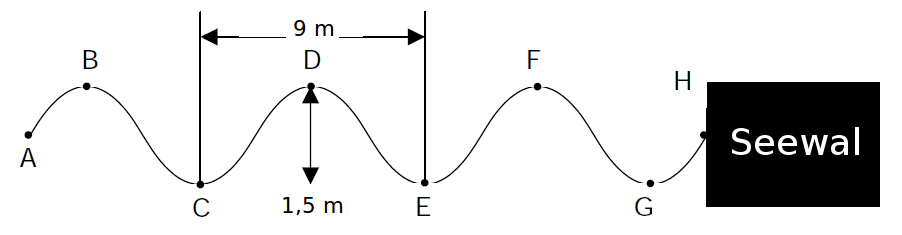
\includegraphics[width=0.8\columnwidth]{col11305.imgs/m38806_seawall.png} % m38806;seawall.png;;;6.0;8.5;
      \vspace{2pt}
    \vspace{.1in}
    \end{center}
 \end{figure}       
\label{m38806*uid081231}\begin{enumerate}[noitemsep, label=\textbf{\alph*}. ] 
            \item Hoeveel volledige golwe word in die skets aangedui?
\item Skryf die letters neer wat enige TWEE punte aandui wat:
\label{m38806*uid0821323}\begin{enumerate}[noitemsep, label=\textbf{\roman*}. ] 
            \item in fase is
\item uit fase is
\item EEN golflengte verteenwoordig.\end{enumerate}
        \item Bereken die amplitude van die golf.
\item Toon aan dat die periode van die golf 0,67 s is.
\item Bereken die frekwensie van die golwe.
\item Bereken die snelheid van die golwe.\end{enumerate}
         \end{enumerate}
  \label{m38806**end}
\practiceinfo
 \par \begin{tabular}[h]{cc}
(1.) 02eb  &  (2.) 02ec  & \end{tabular}

\end{eocexercises}
